%----------------------------------------------------------------------------------------
%
% LaTeX-template for degree projects at LNU, Department of Computer Science
% Last updated by Johan Hagelbäck, Mar 2017
% Linnaeus University
%
% License: Creative Commons BY
%
%----------------------------------------------------------------------------------------

%----------------------------------------------------------------------------------------
%	Settings and configuration
%----------------------------------------------------------------------------------------

\documentclass[a4paper,12pt]{article}

\usepackage[T1]{fontenc}
\usepackage{times}
\usepackage[english]{babel}
\usepackage[utf8]{inputenc}
\usepackage{dtklogos}
\usepackage{wallpaper}
\usepackage[absolute]{textpos}
\usepackage[top=2cm, bottom=2.5cm, left=3cm, right=3cm]{geometry}
\usepackage{appendix}
\usepackage[nottoc]{tocbibind}
\usepackage[colorlinks=true,
            linkcolor=black,
            urlcolor=blue,
            citecolor=black]{hyperref}

\setcounter{secnumdepth}{3}
\setcounter{tocdepth}{3}

\usepackage{sectsty}
\sectionfont{\fontsize{14}{15}\selectfont}
\subsectionfont{\fontsize{12}{15}\selectfont}
\subsubsectionfont{\fontsize{12}{15}\selectfont}
\usepackage{placeins}
\usepackage{csquotes} % Used to handle citations
\usepackage{pythonhighlight}

\renewcommand{\thetable}{\arabic{section}.\arabic{table}}  
\renewcommand{\thefigure}{\arabic{section}.\arabic{figure}} 

%----------------------------------------------------------------------------------------
%	
%----------------------------------------------------------------------------------------
\newsavebox{\mybox}
\newlength{\mydepth}
\newlength{\myheight}

\newenvironment{sidebar}%
{\begin{lrbox}{\mybox}\begin{minipage}{\textwidth}}%
{\end{minipage}\end{lrbox}%
 \settodepth{\mydepth}{\usebox{\mybox}}%
 \settoheight{\myheight}{\usebox{\mybox}}%
 \addtolength{\myheight}{\mydepth}%
 \noindent\makebox[0pt]{\hspace{-20pt}\rule[-\mydepth]{1pt}{\myheight}}%
 \usebox{\mybox}}

%----------------------------------------------------------------------------------------
%	Title section
%----------------------------------------------------------------------------------------
\newcommand\BackgroundPic{
    \put(-2,-3){
    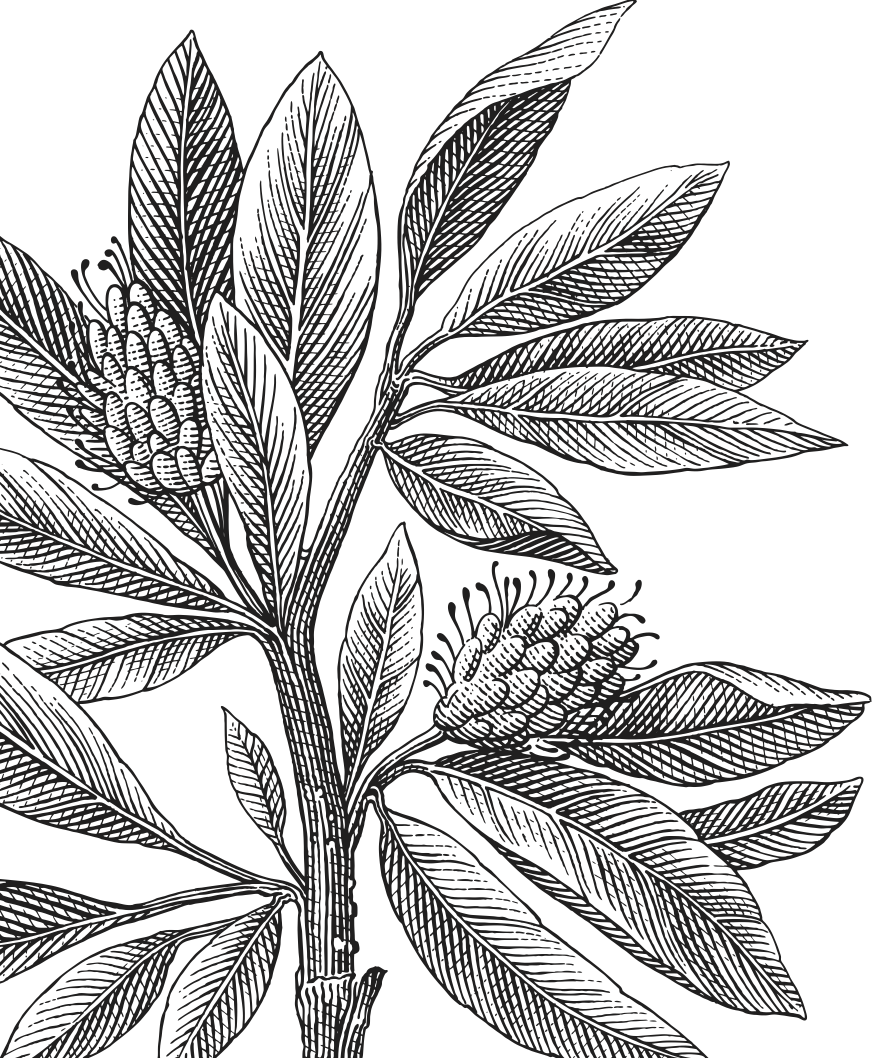
\includegraphics[keepaspectratio,scale=0.3]{img/lnu_etch.png} % Background picture
    }
}
\newcommand\BackgroundPicLogo{
    \put(30,740){
    
\includegraphics[keepaspectratio,scale=0.10]{img/logo.png} % Logo in upper left corner
    }
}

\title{	
\vspace{-8cm}
\begin{sidebar}
    \vspace{10cm}
    \normalfont \normalsize
    \Huge Bachelor Degree Project \\
    \vspace{-1.3cm}
\end{sidebar}
\vspace{3cm}
\begin{flushleft}
    \huge Effective utilisation of DNS Privacy\\ 
    \it \LARGE - Protection towards pervasive surveillance 
\end{flushleft}
\null
\vfill
\begin{textblock}{6}(10,13)
\begin{flushright}
\begin{minipage}{\textwidth}
\begin{flushleft} \large
\emph{Author:} Songho Lee\\ % Author
\emph{Supervisor:} Ola Flygt\\ % Supervisor
%\emph{Examiner:} Dr.~Mark \textsc{Brown}\\ % Examiner (course manager)
\emph{Semester:} VT 2019\\ % 
\emph{Subject:} Computer Science\\ % Subject area
\end{flushleft}
\end{minipage}
\end{flushright}
\end{textblock}
}

\date{} 

\begin{document}
\pagenumbering{gobble}
\newgeometry{left=5cm}
\AddToShipoutPicture*{\BackgroundPic}
\AddToShipoutPicture*{\BackgroundPicLogo}
\maketitle
\restoregeometry
\clearpage
%----------------------------------------------------------------------------------------
%	Abstract
%----------------------------------------------------------------------------------------
\selectlanguage{english}
\begin{abstract}
\noindent Current usage of the DNS system is the most significant loophole of Internet users' privacy, as all queries and answers for resolving web address are not protected in most cases. % Thesis statement, background description
Lack of confidentiality in the DNS system enables everyone who has control of the path between a user and DNS resolver can collect someone's usage pattern and fingerprint him and filter his access to specific websites. % Motivation
Despite a single solution for addressing privacy risks in all stages of the DNS query process does not exist, the report acquaints several Internet standardisations for DNS privacy that are complementary to the existing DNS system and verifies that implementation of these brings significant enhancement of users' privacy.
%The report explores existing methods to enhance DNS Privacy and sets up a series of experiments to verify implementations of such methods for privacy enhancement. % Description of problem explored
\\\\
\textbf{Keywords: DNS, DNS-over-HTTPS, DNS-over-TLS, DNS Privacy}
\end{abstract}

%----------------------------------------------------------------------------------------
%	Preface
%----------------------------------------------------------------------------------------
%\newpage
%\textbf {\large{Preface}}\\

%\noindent You can have a preface in the report if you want, but it is not necessary. In this you can write more personal reflections on your degree project. In the preface you can also take the opportunity to thank the people who have been particularly helpful during the report writing, for example if you had any contact with a company that helped with the project, people that guided or helped you during the project, or your family and friends that supported you during the project. The preface shall not be longer than half a page.

%----------------------------------------------------------------------------------------
\newpage
\pagenumbering{gobble}
\tableofcontents % Table of contents
\newpage
\pagenumbering{arabic}

%----------------------------------------------------------------------------------------
%
%	Here follows the actual text contents of the report.
%
%----------------------------------------------------------------------------------------

\section{Introduction}
This chapter describes what Doname Name System (DNS) is, and how the legacy design of DNS has become a privacy threat. Before discussing the privacy risks of DNS, the background section introduces relevant structure and mechanisms. Knowledgable readers in DNS and Client subnet function may go to section \ref{problemformulation}.

\subsection{Background}
Digital transformation has brought things used to be done in real life decades ago to the online. At work, people have a video conference call instead of a business trip if not necessary. For shopping goods, people fill in credit card numbers for cross-border payments rather than visiting a bank branch to issue paychecks. In other words, the stage where people work now has been shifted to cyberspace in recent decades, and the Internet has become an essential part of everyday life.

Despite the ubiquitousness of the Internet, users' activities online are collected under pervasive monitoring by different actors.
Pervasive monitoring means ``widespread attack on privacy \cite{rfc7258}.'' Information collected in such action could lead to a breach of users’ privacy, by re-identifying users based on traffic \cite{herrmann2010analyzing}, or could become aids for launching an active form of attacks, such as masquerade and Denial of Service (DoS).
Unfortunately, the insecure architecture of Domain Name System allows the pervasive monitoring, and thus it should be mitigated. Before discussing the privacy problems of DNS, we introduce DNS and its components which are important to address.

\subsubsection{DNS}\label{dns-introduction}
Every activity on the web most likely begins with entering a human-friendly domain name in the web-browser. Once we enter a domain name for visiting a website, DNS resolves the address to an actual Internet Protocol Address of a web server which hosts the website. In case multiple websites are hosted on a single server, the entered fully qualified domain name(FQDN) is used to differentiate virtual hosts on a web server \cite{virtual24host}. Therefore, DNS is a critical component of the Internet.
%What about describing hjierarchical structure of Domain Name System here?
\subsubsection{DNS Servers}\label{dnsservers}
DNS servers consist of four types: Stub resolver, Recursive resolver, Authoritative server, and Forwarding DNS server. Resolvers refer to programmes that obtain information from name servers upon clients' requests \cite{rfc1034}.

Stub resolver is a resolver that serves as an entry-point of querying DNS from applications and directs search request to the nearest recursive resolver \cite{rfc1123}. As it cannot complete domain name resolution by itself, stub resolver is dependant on a recursive resolver \cite{rfc8499}.

The recursive resolver is a server which receives a DNS query from a stub resolver and gets the final answer to the query, by (1) answering from its local cache or (2) sending queries to other DNS servers \cite{rfc8499}. After a recursive resolver has sent a query request to other authoritative name servers, it is expected for the resolver to store the answer as a \textbf{local cache}. It is the first server in DNS query flow that contacts other servers to get the answer for the client. 

Authoritative (name) server is a server that has ``authority over one or more DNS zones \cite{rfc8499}'' and ``can answer queries without needing to query on other servers as it knows the content of the queried DNS zone by local knowledge \cite{rfc2182}.''

DNS forwarding server is a server that forwards queries to recursive resolver or other forwarding servers. It does not perform a query process for the stub resolver.
\subsubsection{DNS Query process}
Due to the hierarchical structure of the Domain Name System with delegations of authorities \cite{rfc1591}, getting the exact IP address of a given domain name involves several DNS servers. Figure \ref{queryprocess} shows an example of querying ``saimei.ftp.acc.umu.se.''. 
\begin{figure}[ht!]
    \begin{center}
        \includegraphics*[width=\columnwidth]{img/dnsquery}
    \end{center}
    \caption{DNS Query sequence diagram}
    \label{queryprocess}
\end{figure}
In the diagram, steps 2 and 3 returns top-level-domain(TLD) from the root servers. The steps 4 and 5 obtain the Authoritative name server of Swedish TLD. The .SE TLD returns name server of Ume\aa\ University in steps 6 and 7. In the last, the name server of umu returns IPv4 address (A record) of the given address, so that recursive resolver can provide the answer to the stub resolver. These steps are performed under the assumption that none of the queries is cached. 
\subsubsection{EDNS(0) and Client Subnet}
The extension mechanisms for DNS (EDNS) is specified in RFC 6891.
EDNS allows both DNS servers and client to send ``larger DNS packet than the original 512 octet limit \cite{rfc6891}'' so that it benefits of utilising larger size.
It makes sending long IPv6 address and possible DNSSEC signatures.
As of February 2019, major DNS resolver operators have started not to support non-EDNS compliant servers \cite{dns-flag-day, spacek-edns-camel-diet}. 

EDNS(0) provides several options, and one of the options is Client Subnet(ECS) feature, as described in RFC 7831 \cite{rfc7871}. When ECS is used, recursive DNS servers provide a truncated client IP address in its DNS queries to the upstream authorities to permit ``topologically localised answers for Content Delivery Networks (CDN) \cite{kintis2016understanding}''.
\subsubsection{CIA-triad}
In information security discussions, threat mitigations of a system are analysed in three perspectives: confidentiality, availability and integrity. These properties as a group are denoted as CIA triad or the security triad.
Achieving every aspect of CIA-triad often are not feasible, as enhancing one dimension may interfere with the other dimensions \cite{securityincomputing}.


\subsection{Related work}
The project accredits pioneer research of ``DNS Privacy Considerations (RFC 7626) \cite{rfc7626}'' which has provided theoretical foundations in analysis of DNS privacy. 
As of 2019, there are several studies presented to mitigate privacy issues based on the analysis. These studies are later presented in Chapter \ref{surveyresults}.

P. Werneck and J.H.C. van Heugten presented surveys of DNS privacy-enhancing methods. P. Werneck evaluated approaches to improve the privacy of DNS and stated the limitations of identified approaches \cite{werneck2014dns} in 2014. J. Heugten evaluated existing solutions to enhance DNS Privacy in 2018 in his study \cite{van2018privacy}. As standardisation of DNS-over-HTTPS is recently finalised \cite{rfc8484}, a study from van Heugten reflects more recent changes.

\subsection{Problem formulation}\label{problemformulation}
Currently, almost all DNS traffic is sent in clear text \cite{rfc7626} over the UDP protocol \cite{tcp2014analysis}, and it makes DNS queries vulnerable to being hijacked or used to filter users' traffic.
All participants of the DNS query process, as illustrated in Figure \ref{queryprocess}, transmit messages intensively, and these are in plaintext.
It is also noteworthy that all participating authoritative name servers receive the same questions, although it is not necessary for Authoritative servers in higher hierarchies in the process to know all the complete domain address in question.

S. Bortzmeyer has analysed that particular fields in DNS packet \cite{rfc1035} such as Query name (QNAME) and Source IP address reveal ``communication relationships \cite{rfc7626}''.
These series of observations indicate that there are risks of information leakage in following places: (1) tapping on the wire ``between the stub resolvers and the recursive resolvers'', and (2) information leaks in the servers.
The following research questions are formulated having regards to the privacy breaching circumstances.

\begin{table}[h!]
    \begin{tabular} {|p{1.2cm}|p{12.8cm}|} \hline
        \textbf{RQ1} & Which benefits would DNS Privacy bring to different parties? \\ \hline
        \textbf{RQ2} & Which are the use cases that the exisiting DNS Privacy enhancement methods could not address? \\ \hline
        \textbf{RQ3} & Which combination of technologies would be suitable to address the limitation of the current status?\\ \hline
    \end{tabular}
    \caption{Research questions}
\label{researchquestions}
\end{table}

\subsection{Motivation}
Most of the internet activities begin with DNS query, hence DNS is vital. Notwithstanding the importance of DNS, designers of the current DNS protocol have not taken consideration of ``confidentiality of protocol metadata'' \cite{wachs2014censorship}.
Therefore DNS queries reveal communication flows, and this property of DNS protocol is used in different contexts by different actors. Examples of usages are traffic monitoring for network management or limiting the influence of malicious websites by DNS Footprinting of malware \cite{stoner2010dns}, or detecting malware infections \cite{lemos2013got}.

Other exemplary usages of this property of DNS are nation-state surveillance \cite{NSA-SIGINT}, privacy-unfriendly activities of commercial sectors \cite{weaver2011redirecting}, and illegal actions by criminals. Surveillance affects individuals to possess stress and anxiety \cite{oulasvirta2012long}, and behavioural changes like self-censorship \cite{rfc6973}. RFC 6973 connotes that Privacy harms involve ``harms to financial standing, reputation, solitude, autonomy, and safety \cite{rfc6973}'' of individuals.

S. Farrell et al. state in RFC 7258 that allowing monitoring by benevolent actors and defending privacy against nefarious actors do not hold hand in hand, as the actions required to achieve both, regardless of the motivations, are indistinguishable \cite{rfc7258}.
Disadvantages incurred by lack of DNS privacy significantly overweight advantages, and therefore DNS privacy should be mitigated in any feasible practices.

\subsection{Objectives}
The following objectives are set to answer the research questions and transform the tasks into the smaller pieces, and reasonings on each objective follow below. Hereafter several words are shortened for the ease of denotation, such as an objective as O and a research question as RQ. Table \ref{objectives} summarises the objectives.
\begin{table}[h!]
    \begin{tabular} {|p{1.2cm}|p{12.8cm}|} \hline
        \textbf{O1} & Analyse different end-users' privacy infringements when not having DNS Privacy\\ \hline
        \textbf{O2} & Explore the state of arts in mitigative methods to enhance DNS Privacy \\ \hline
        \textbf{O3} & Identify areas which the selected methods could not address. \\ \hline
        \textbf{O4} & Analyse alternative approaches to mitigate the current limitations.\\ \hline
    \end{tabular}
    \caption{Objectives}
    \label{objectives}
\end{table}

RQ1 aims to explore benefits by having DNS privacy on a different group of people.
As it could be challenging to motivate benefits of having privacy when obscurity prevails, O1 is defined to analyse scenarios when the privacy is violated caused by having insecure or exposed DNS queries.

RQ2 is to find use cases of the existing DNS privacy mitigative methods. However, in order to discuss use cases, the state of these methods need to be examined. Therefore, O2 is set to explore the state of arts of the methods and O3 is set to identify areas for  improvements.

RQ3 attempts to provide useful interventions by finding a combination of technologies to overcome the limitation of the current DNS Privacy enhancement. For serving the purpose, O4 discusses possible approaches to using other technologies.

\subsection{Scope/Limitation}
The project has a focus on improving the privacy part, from the security perspectives. In other words, reflected to a Confidentiality, Integrity, Availability(CIA) triad, enhancing Integrity and availability perspectives are less prioritised in the current project. Issues and challenges of DNS security as a whole may be found in other studies, such as one conducted by Ning Hu et. al.\cite{ning2017dnssecurity}. 

\subsection{Target group}
The project aims to provide insight on DNS Privacy for Internet users and recursive resolver providers for improving users' privacy.
%Here you outline which target group that might be interested in your work. If you, for example, do a project about software architectures, a target group can be professional developers and architects that work with similar software systems as the system you investigated.

\subsection{Outline}
The majority of scientific reports follow in Introduction, Methods, Results, Analysis and Discussion(IMRaD) pattern. However, the project chose to use a design science method and therefore it has an inverted structure of results and analysis. An analysis is made first to describe the design constraints and results (or design proposal) are presented afterwards. 

\newpage
\section{Method}\label{Method}
This chapter describes the chosen scientific methods to answer the research questions (Table \ref{researchquestions}) and meet the objectives (Table \ref{objectives}).
The study used scientific methods of systematic literature review and design science. Controlled experiments were also partially used to verify several statements made in the study. Sections follow to motivate the choice of a scientific method for meeting objectives.
\subsection{Systematic literature review}
A systematic literature review was performed to accomplish O2, which is to study mitigative methods of DNS privacy. Although a recently published article provided an overview of DNS Privacy enhancing methods \cite{van2018privacy}, performing systematic literature review was necessary to eradicate possible biases and to minimise opportunities of missing suitable solutions.

A search criterium was set to list articles that cited RFC 7626 from a database Google Scholar to make the review process systematic. RFC 7626 is chosen, as its analysis had provided a clear insight of DNS privacy issues \cite{rfc7626}, and since around four years had passed after its publication, it was anticipated that fellow researchers have tried to solve or list risks identified in the article.

For inclusion criterium, references of the found articles were further examined, as there were chances of missing to address well-established solutions possibly because the methods had been introduced before publishment of RFC 7626.

Exclusive criteria were set to have the contents of the articles to be relevant to the defined problem. Therefore, any solving other security aspects of DNS, such as availability but not addressing the privacy problems were excluded.

\subsection{Design Science}
Design science ``creates and evaluates Information Technology artefacts to solve identified organisational problems \cite{von2004design}'', and it has strong relevance in addressing O3 and O4 which are to identify the area that studied DNS Privacy methods could not address and analyse alternative approaches to overcome the limitations.

To refine problem statements for the existing practice, a literature review is made to analyse privacy infringement scenarios on diverse user scenarios, as defined in O1.

\subsection{Controlled Experiment}
A controlled experiment is applied to verify whether the suggested design artefact addressed the limitations of current DNS Privacy enhancing methods found in O3 or not. Conducting a controlled experiment fulfils one of the guidelines of design science which requires ``thorough evaluation of the artefact \cite{von2004design}''.

\subsection{Reliability and Validity}
The study is seen to have reliability on the results of the literature review, as the same effect will be derived by performing a search as described in the previous section. As Appendix A includes the source code of the experiment scripts, a similar result is expected to be derived by other researchers as well. 

The project deployed its experiments in a virtualised environment to minimise unforeseen factors that would impact performance measurements.

\subsection{Ethical considerations}
Discussing ethical considerations has less significance in the chosen methods, as no real data of any physical persons is collected without the consent.
However, it can be questioned whether it is adequate to elaborate privacy breaching scenarios in details to use the information for formulating problems for the design science method.
Despite the concerns, as the project aims to improve the problematic scenarios of not having sufficient privacy enhancements, describing the problematic situations as-they-are is necessary.

\newpage
\section{Privacy profiles}
Privacy is seen as having an access control in confidentiality in a security domain.
In everyday language, Privacy means ``the right to control who knows certain things about you \cite{securityincomputing}''.
Pfleeger introduces three aspects of Information security: sensitive data, affected parties, and controlled disclosure.
Privacy issues related to the DNS on different subjects are analysed in this chapter.

\subsection{Affected subjects}
The subjects are classified as private persons, and organisations. Organisations are further divided into large organisations that operate their directory server with DNS, and the smaller organisations that do not operate DNS resolvers in its network.

\subsection{Sensitive information}\label{sensitiveinformation}
Defining what sensitive information is in a subjective area.
Therefore, sensitiveness of the information cannot be measured on an absolute scale. However, several common areas of sensitive information follow.

For natural persons, EU has defined sensitive information as the following: personal data revealing ``(1) ethnic origin, religious or philosophical beliefs, (2) trade-union membership, (3) health-related data, and (4) data concerning a person's sex life \cite{GDPR}''.

For organisations, of their information, assets, especially copyright (expression of the idea), trade secret, and privileged information are examples of sensitive information \cite{securityincomputing}.

\subsection{Controlled disclosure}
The information has a different characteristic compared to any physical asset; it can be duplicated to an infinite amount at relatively low cost, without harming the asset.
This unique characteristic of information makes a ``propagation problem''.
Affected subjects lose control of the information about themselves after being disclosed.

\subsection{Privacy breaching Scenarios}
This section provides an analysis of the privacy breaching circumstances per affected subjects by observing DNS. Before focusing impacts on each subject, common privacy impacts are introduced by elaborating the privacy-related metadata.
Bortzmeyer highlighted that ``DNS data itself and a particular transaction'' should be confidential and transaction should not be public \cite{rfc7626}. The transaction refers to the DNS lookup in this context.
The following sections demonstrate how DNS reveals sensitive information about the affected subjects.

\begin{figure}[ht!]
    \begin{center}
        \includegraphics*[width=\columnwidth]{img/privacyobject}
    \end{center}
    \caption{Privacy related components on DNS transaction}
    \label{privacyobject}
\end{figure}

\subsubsection{Metadata in DNS query}\label{dnsmetadata}
Figure \ref{privacyobject} identifies relevant metadata created on DNS transaction.
The metadata created when looking up DNS record includes Query Name (QNAME or Request Name), Query type and client's IP address.
Contrary to the belief that metadata has only minimal information, the client IP address can be linked with WHOIS \cite{whois-icann}. Furthermore, geographical information of the client and affiliate of the organisation can be derived.

The recursive resolver can see whether the query is answered from its cache or not, and this information provides an insight into the client's behaviour.
Given a sufficient number of clients sharing the same recursive resolver, ``DNS queries on Chinese Top-Level-Domains(TLD) server had Zipf-like distribution \cite{wang2013analysis}''. If this phenomenon also applies to the rest of the TLDs, administrators of the recursive DNS resolver could infer that a user attempts to visit not-so-frequently-visited web server.

\subsubsection{Impact on individuals}
The Sensitive information related to the individuals can be derived by observing metadata created on DNS lookup process. The example scenarios are given in the order of information defined in section \ref{sensitiveinformation}.

There may be a domain shared mainly by people with shared philosophical beliefs if people are situated in countries with the legislation of censoring obligations on websites' administrators.
It is likely that people that share certain philosophical or political beliefs would host a dedicated website for holding a community rather than utilising censorship-enabled large social platforms \cite{mackinnon2009china}.
In such case, when a person visits such website, it may provide sufficient signal of the user's philosophical beliefs to those who can eavesdrop the traffic, although the detailed activities on such website are protected by encryption.

An employee visiting a certain trade-union's website frequently in a corporative network may indicate to an IT-department that either the person is a member of the union or has a sympathy with the organisation. 

Observing DNS query enables deriving health-condition of a user. If a chronic disease patient bears a smart sensor (such as Continuous Glucose Monitoring) that securely sends the measurement data to medical institutes \cite{carelink-uploading, medtronic-watson}, observing her DNS traffics may infer his health condition.
If someone actively visits several clinics that specialise in a particular disease and relevant medical insurance company's website, consequent DNS queries provide meaningful insight into the person's health status.

DNS queries related to online dating sites can also be observed. However, there has not found any evidence of potential sexual activity of individuals based on the frequency of the visit, without considering its sociosexuality \cite{sevi2018exploring}. 
Although the sexual activity cannot be derived, the sexual orientation of individuals could be induced in case the queried address is mainly visited among sexual minorities such as Grindr - the gay dating app \cite{goedel2015geosocial}.

\subsubsection{Impact on corporates/organisations}
The section illustrates privacy breaching scenarios for corporates' interest. First, scenarios of a large organisation are described. A common scenario regardless of the size of the organisations follows afterwards.

Assuming that large-scale enterprises have sophisticated intranet and employees are assigned with managed work laptops, an employee would utilise a web browser's bookmark to add company specific websites on his work computer.
In this case, although users do not necessarily visit the corporative intranet sites, a web browser may prefetch the bookmarks \cite{firefox-autocomplete-url, chrome-dns-prefectching}, which in its turn leaks the DNS queries.
If the employee was travelling, the leaked domain names have potentials to reveal employee's identity in public places by any observers, and the domain names can be collected to facilitate sophisticated and active attacks in the future.
In addition to the leaks caused by bookmarks from the browser, a query value `\textunderscore ldap.\textunderscore tcp.hostname' indicates that a client's dependency of a directory server \cite{Shulman:2014} and reveals the existence of service in the hostname.

Activities on new product development or sensitive assignment may be derived from the DNS query activities originated from the corporative IP address. Section \ref{dnsmetadata} mentioned about WHOIS record of IP addresses. Information on Autonomous System (AS) - administrative entity - might have a more substantial impact on identity linking on corporates compared to the individuals, once the information is correlated with the content of DNS Queries and frequency of the queries. Exchanging e-mails among various organisations or clients also involves DNS resolution and in this case Query type matters, since mail exchange server information is fetched by MX record of the DNS.

\subsection{DNS queries as a digital fingerprint}\label{fingerprint}
Kirchler et al. discuss possible ``behaviour-based-tracking'' of linking user sessions with the help of unsupervised learning of their DNS traffic patterns \cite{kirchler2016tracked}. Potential usage of such technique may especially be alarming for members of an organisation with critical missions, not only the private individuals.
Alongside with Kirchler's study, having an assumption that users would not change their recursive DNS resolver frequently, end-user reidentification based on web browsing history patterns \cite{olejnik2012johnny} could also be applicable in the context, as observing DNS query traffic provides a good representation of each client's web browsing history.

\newpage
\section{Survey of DNS Privacy enhancing methods}\label{surveyresults}
This chapter presents the result of a systematic literature review on studies related to DNS Privacy.
%Afterwards, the analysis of the result follows.
As the raw data from the Google scholar had contained several duplicated entries, duplicated studies were excluded. Series or revisions of the same article are marked as duplicated. For such cases, the proceeding study was chosen to present.
The analysis section which follows after this chapter motivates strategies for categorisation of raw search results.

\subsection{Improvement suggestions}
Studies shown in Table \ref{channel} attempted to secure the communication channel of the DNS query. In other words, these studies suggested applying Encipherment mechanism to deliver Connection Confidentiality as X.800 defines \cite{x800}.

\begin{table}[h!]
    \begin{tabular}{ | l | p{10.5cm} | l | l | }
        \hline
            ID & Title & Year & Cites  \\ \hline
            \cite{hu2016specification} & Specification for dns over transport layer security (tls) & 2016 & 27 \\ \hline
            \cite{rfc8484} & Dns queries over https (doh) & 2018 & 5\\ \hline
            \cite{reddy2017dns} & Dns over datagram transport layer security (dtls) & 2017 & 3\\ \hline
            \cite{bucuti2015opportunistic} & An opportunistic encryption extension for the DNS protocol & 2015 & 2 \\ \hline
            \cite{dickinson2018usage} & Usage profiles for dns over tls and dns over dtls & 2018 & 1 \\ \hline
            \cite{saraj2017design} & Design and implementation of a lightweight privacy extension of DNSSEC protocol & 2017 & 0 \\ \hline
            \cite{dnsoquic} & Specification of DNS over Dedicated QUIC Connections & 2019 & 0 \\ \hline
            \cite{denis2015dnscrypt} & DNSCrypt & 2015 & 0 \\ \hline
            \cite{dempsky2010dnscurve} & DNSCurve & 2009 & 0 \\ \hline
        \end{tabular}
        \caption{Literatures categorised as securing communication channel}
\label{channel}
\end{table}

Table \ref{content} summarised studies on minimising privacy breaching information in the content of packets generated in the DNS query process.
%The approach can be seen as metaphors of Least common mechanism and Isolation as described in security design principles. 

\begin{table}[h!]
    \begin{tabular}{ | l | p{10.5cm} | l | l |}
        \hline
            ID & Title & Year & Cites \\ \hline
            \cite{bortzmeyer2016dns} & DNS query name minimisation to improve privacy & 2016 & 33 \\ \hline
            \cite{annee-dprive-oblivious-dns-00} & Oblivious DNS - Strong Privacy for DNS Queries & 2019 & 0 \\ \hline
            \cite{pan2018mitigating} & Mitigating Client Subnet Leakage in DNS Queries & 2018 & 0 \\ \hline
        \end{tabular}
        \caption{Literatures categorised as securing content}
\label{content}
\end{table}

There are several pieces of research and design proposals of new architecture which would replace the current DNS system. These are found in Table \ref{architectures}

\begin{table}[h!]
    \begin{tabular}{ | l | p{10.5cm} | l | l | }
        \hline
            ID & Title & Year & Cites \\ \hline
            \cite{ambrosin2018security} & Security and privacy analysis of national science foundation future internet architectures & 2018 & 3 \\ \hline
            \cite{grothoff2017gnunet} & The GNUnet System & 2017 & 1 \\ \hline
            \cite{asoni2017paged} & A Paged Domain Name System for Query Privacy & 2017 & 0 \\ \hline
            \cite{loibl2014namecoin} & Namecoin & 2014 & 12 \\ \hline
        \end{tabular}
        \caption{Literatures categorised as Architectural proposal}
    \label{architectures}
\end{table}
\FloatBarrier
\subsection{Case studies on attack scenarios}
Several studies demonstrated privacy risks of the current DNS standard and proposed mitigative methods which we had introduced in the previous section. 

\begin{table}[h!]
    \begin{tabular}{ | l | p{10.5cm} | l | l | }
        \hline
            ID & Title & Year & Cites \\ \hline
            \cite{kirchler2016tracked} & Tracked without a trace: linking sessions of users by unsupervised learning of patterns in their DNS traffic & 2016 & 10 \\ \hline
            \cite{mohaisen2017leakage} & Leakage of. onion at the DNS Root: Measurements, Causes, and Countermeasures & 2017 & 3 \\ \hline
            \cite{grothoff2017nsa} & NSA's MORECOWBELL: knell for DNS & 2017 & 3 \\ \hline
            \cite{spaulding2018d} & D-FENS: DNS filtering \& extraction network system for malicious domain names & 2018 & 1 \\ \hline
        \end{tabular}
        \caption{Literatures categorised as demonstrating attack scenarios by exploiting the lack of DNS privacy}
\label{attacks}
\end{table}

\newpage
\section{Analysis of DNS Privacy enhancing methods}
This section provides an analysis of the survey results.

Classification of DNS Privacy methods could further be analysed based on the which privacy risk these address. S. Bortzmeyer identified risk area of DNS privacy in RFC 7626 as the followings \cite{rfc7626}: 
\begin{enumerate}
    \item Data in the DNS request
    \item On the wire
    \item In the servers
    \item Re-identification and other Interferences
\end{enumerate}
Following sections analyse privacy risk mitigations based on risk area and type of mitigation strategies as a whole. Concent, privacy and performance analysis of each mitigative method can be found in \cite{van2018privacy}.

\subsection{Two phases of DNS Query process}
For the conciseness of further analysis, the communication channel (transport channel) of DNS are abstracted into two phases or paths based on the DNS Query process.

\textbf{Phase 1} refers to step 1 and 10 of Figure \ref{queryprocess}. These two steps are performed in the DNS Query process when stub resolver queries a domain name to the recursive resolver and the recursive resolver replies to the stub resolver.
Channel-wise, it is denoted as a \textbf{stub-to-resolver link}.

\textbf{Phase 2} refers to the steps in the Figure \ref{queryprocess} where a recursive resolver finds the final answer to the queried address, by recursively reaching to concerning authoritative servers. In other words, the channel that the rest of the steps is performed is called \textbf{recursive-to-auth link}.

\subsubsection{Insufficient measurements on recursive-to-auth link}
The distinction of the two phases are noteworthy, as the current implementations that preserve DNS hierarchical structure do not secure all communication paths towards all involved parties of the DNS resolving.
As an example, the majority of the methods do not encrypt communications on Phase 2 (recursive-to-auth link) in contrast to Phase 1 (stub-to-resolver link).
The fact that an authoritative server having a one-to-many server-client relationship from the recursive resolvers is the major obstacle of applying encryption on Phase 2.

As a further explanation of one-to-many relationship being an obstacle, DoH \cite{rfc8484} and DoT \cite{hu2016specification} use Transport Layer Security (TLS) protocol \cite{rfc7858} for encryption. In the case an authoritative server process multiple TLS session, it is likely to end up exhausting its computational resources \cite{bhople2012server}, similar to a Distributed DoS (DDoS) attack situation. The internet draft ``Next step for DPRIVE: resolver-to-auth link \cite{I-D.bortzmeyer-dprive-step-2}'' discusses the aforementioned challenges.

Furthermore, authentication mechanisms are missing on Phase 2 \cite{I-D.bortzmeyer-dprive-step-2}, and the lack of authentication of the authoritative server may potentially enable a Man-in-the-middle attack (MITM).
Therefore, the location of the DNS resolver needs to be considered when to mention the limitations of each suggested methods.
% There are proposal of utilising TLS 1.3 and 

\subsubsection{Location of Recursive DNS resolvers}
From the end user's point of view, recursive DNS Resolvers can be on a local machine, one provided by the Internet Service Providers (ISP) and Public DNS servers \cite{van2018privacy}.
Selection of the location of recursive DNS resolvers leads to different impacts on the user's privacy, in terms of cache-sharing\cite{van2018privacy, wang2013analysis} and obfuscation and logging. Section \ref{dnsservers} described caching on recursive resolvers.

\begin{figure}[ht!]
    \begin{center}
    \includegraphics*[width=0.9\columnwidth]{img/local-recursive}
    \end{center}
    \caption{A simplified network map when using local resursive resolver server.}
    \label{localrecursive}
\end{figure}
When a user utilises a \textit{local recursive resolver} as illustrated in Figure \ref{localrecursive}, channel encipher methods do not add value to users' privacy considering that operations of phase two are often not encrypted.
Supposing that the user does not share local recursive resolver among the others, DNS queries which the user makes will not be fetched from a cache but, instead, from all involved Authoritative Name Servers (NS).
Sending queries in clear text on phase 2 leaves a possibility for all parties who are involved in the network packet transmission to monitor QNAME, query type and source IP of the traffic towards authoritative NS.
Referring to the assumption that local recursive resolver is unique for a person, there is no space for obfuscation since no one else is querying from the IP address of the recursive resolver.
However, utilising the local recursive resolver eliminates the risks of queries being logged (i.e. (3) risk in-the-servers) during Phase 1.


\begin{figure}[h!]
    \begin{center}
    \includegraphics*[width=0.9\columnwidth]{img/isp-recursive}
    \end{center}
    \caption{A simplified network map when using ISP-provided resursive resolver server.}
    \label{isprecursive}
\end{figure}
Using \textit{ISP provided Recursive resolver} is the most common scenario, as most ISP offer DNS resolver to their users by Dynamic Host Configuration Protocol (DHCP).
The resolver from ISP is shared with other subscribers of the network, and it increases more chance of having queries cached by another user who acquired the address previously.
Reusing cache reduces the need of Phase 2 in its response process \cite{wang2013analysis} and thus generates less `often-insecure' traffics towards authoritative NS. 
Authoritative name servers see the source IP address of ISP's resolver in Phase 2 of DNS resolving, but not IP of the individuals, in case E-DNS Client Subset(ECS) is not in place.
When ECS is used, the authoritative NS may see truncated IP of clients \cite{kintis2016understanding}, but the IP address does not present additional privacy harm as ISP's recursive resolver is often in the same subnet IP range, and authoritative NS already acquaints source IP of the recursive DNS resolver. 
Privacy risks incurred by logging may exist in ISP provided resolver, as ISPs may be obliged for log retentions due to legal requirements of the countries they operate in.
Channel encipherment on Phase 1 adds a value of users' privacy to a limited extent, tapping on the wire between the ISP's recursive resolver and a stub resolver is often feasible for ISP itself rather than third parties.

\begin{figure}[h!]
    \begin{center}
    \includegraphics*[width=0.9\columnwidth]{img/public-recursive}
    \end{center}
    \caption{A simplified network map when using public resursive resolver server.}
    \label{publicrecursive}
\end{figure}

A scenario of using a \textit{public recursive resolver} (as known as Public DNS resolver) is represented in Figure \ref{publicrecursive}.
A public DNS server has more possibilities of being shared by a broader public compared to the ISP provided resolvers, and it increases the chances of queries being already cached. Authoritative servers see requests from the IP address of the public resolver, instead of stub resolvers' when ECS is not applied.

This scenario benefits users the most when channel encipherment is applied because DNS query contents in Phase 1 is not visible for parties in the middle of the networking path. It brings significant obfuscation in tracking down the end-user by analysing the network traffics. However, Public DNS servers may log the DNS queries and information of the client. Therefore, privacy risk in-the-servers remains.

\FloatBarrier

\subsection{Prevalence of hierarchical DNS}
Although the primary focus of the study is made on Domain Name resolving part, DNS resolving is only a portion of the entire DNS, as there are diverse actors (such as administrators, domain owners) involved in the system.
Figure \ref{dnsactors}, which is presented by SUNET \cite{SUNET-DNS}, illustrates the involved machines and servers of the system as a whole.

\begin{figure}[h!]
    \begin{center}
    \includegraphics*[width=1\columnwidth]{img/DNS-maskinvara}
    \end{center}
    \caption{Parties involved in DNS as a whole \cite{SUNET-DNS}}
    \label{dnsactors}
\end{figure}

In the figure, sections are vertically divided.
The figure in the first column represents organisations or individuals that desire to acquire a new domain name.
The third column of the figure demonstrates administrators of delegation on each autonomous domain hierarchy.
Legacy of the system are often neglected in attempts of securing the domain name resolution process, which is presented in green colour in the figure. 

The naming hierarchy of the DNS ``ties into systems such as the Public Key Infrastructure (PKI) \cite{akamai-dns-architecture}'', and architecture of decentralised DNS, such as NameCoin \cite{loibl2014namecoin}, may have not considered the PKI structure in its design.

\subsubsection{Privacy analysis of Namecoin}
Preserving user privacy in Namecoin requires ``replication of the full blockchain at the user's end system \cite{grothoff2017nsa}'' and performing such received a criticism that it ``may be impractical for some devices \cite{grothoff2017nsa}.''
The criticism can be interpreted as applying blockchain did not add significant value, in terms of preserving the privacy of users, as privacy breaches in DNS resolving process could also be addressed if DNS records could be replicated on a client's system even in the existing hierarchical system. 

\subsubsection{Privacy analysis of GNS}
Authors of the GNS claim that domain resolving process of the GNS is private because ``queries and responses are encrypted \cite{grothoff2017nsa, wachs2014censorship}.''
However, its confidentiality is vulnerable for `confirmation attack' if ``the adversary knows both the public key of the zone and the specific label \cite{wachs2014censorship}.'' Note that the label refers to an entry in a petname system. 

\subsubsection{The integrity of the DNS records}
Ensuring the integrity of the DNS record is significant, and it is evident from `phishing attacks \cite{ariyapperuma2007security, ollmann2004phishing}'.
Per contra, radical protocol design proposals may harm the integrity of the DNS records, as its proof-censorship or legal-attack-proof designs may enable everyone can claim the legitimacy of ownership of the specific domain.

Solutions using DHT in its design may put the system vulnerable to possible Sybil attacks \cite{6503215, SitE2002Scfp}.
Sybil attacks are a type of attack scenario where an attacker `subverts the reputation system by creating a considerable amount of pseudonymous identities \cite{TRIFA20141135}' `in the absence of identification authority \cite{douceur2002sybil}.'

Interventing the malvaceous records are more challenging than the hierarchical structure of the current DNS system in the decentralised design, and this could lead to concerns of enabling phishing attacks.
Enhancing confidentiality aspects of DNS security is important but it should not compromise the integrity aspect.



\subsubsection{The availability of the DNS Service}
There are several criteria to define availability. The criteria for defining availability introduced by Pfleeger are (1) having a timely response to a given request, (2) ensuring fair allocation of resources and (3) being fault-tolerant \cite{securityincomputing}.
This report defines availability as a chosen recursive resolver to resolve the queried address and provide the correct IP address promptly.

High availability of DNS is important since web activities cannot be initiated without name resolution (as mentioned in Section \ref{dns-introduction}). High performance (performance refers to having a low latency) of DNS is also an important factor to consider because DNS resolutions are a significant cause of having log Web waits \cite{cohen2003proactive, jung2002dns}, and it has a notable impact on `User-perceived latency'.

However, security concerns arise in terms of availability for Oblivious DNS, as ODNS operations require ODNS-stubs and imposing such design creates a new `central point of failure \cite{minutes-102-dprive}'.
Also, questions concerning assuring confidentiality of the keys used in ODNS and issues with fallback have not been answered \cite{minutes-102-dprive}.



\subsection{Privacy leaks by Transitive trust}
Shulman demonstrated that `straightforward application of the encryption alone may not suffice \cite{Shulman:2014}' for protecting DNS Privacy due to possible disruption of DNS Availability and privacy leaks caused by `transitive trust \cite{Ramasubramanian:2005}'.
Shulman further analysed transtive trust as (1) \textit{fan-out} and (2) \textit{chain-length}.
Chain-length refers to ``A number of name servers involved in a resolution of a record that initiates the chain'' and fan-out as ``number of (transitive-trust) chains involved in a resolution of a domain name'' \cite{Shulman:2014}.

Transitive trust at authoritative servers possess a potential risk of revealing the query and client. While DNS QName minimisation \cite{bortzmeyer2016dns} limits the scope of the query name leaks, the extensified usage of DNS in Content Delivery Network (CDN) context \cite{WANG2018235} may have increased the chain-length and it leads to the intercoperation issues \cite{Huque-QNAME-Min-analysis}.

\subsection{Observation on packets' size}


\newpage

\section{Proposal}
This chapter describes the product of the study, considering the analsys made in the previous chapters and given constraints.

\subsection{Non-trusted recursive resolver}
When a trustable recursive resolver does not exist, offen end-users' own computer becomes the recursive resolver. However, the earlier chapter analysed that utilising recursive resolver on a local machine barely gives any value, because many of recursive-to-auth links are unencrypted and subject to the traffic monitoring.

To circumvent the situation, traffic anonymisation technologies on recursive-to auth link can be applied, and examples of such technology are  FreeNet \cite{clarke2001freenet} or GNUNet\cite{grothoff2017gnunet}, and Tor.
However, FreeNet \cite{clarke2001freenet} or GNUNet \cite{grothoff2017gnunet} result in having high delays \cite{anonymousoverdns}.

Solution: Proactive caching \cite{cohen2003proactive} over Tor for most significantly visited websites. For caching, the same tor circut can be reused but for processing individual queries, connection shall not be resued.

Variation of Round Trip Time and its impact on the end-user's perseption shall be discussed. Intercoperation problem with CDN follows.
Provide Privacy analysis on the Tor. Tor may still be subject to the confirmation attacks, similar to DHT technologies. 

Tor cannot forward UDP traffic on the exit-node. (Citation needed). Therefore, it may be difficult to argure the planned idea.
Instead, try to combine DNS-over-TLS or DNS-over-HTTPS with Tor over its proxy socket \cite{tor-socks}, and try to use a DNS resolving client such as \cite{technitium-configuration}. 
\newpage
	
\section{Discussion}
The project intensively examines securing Domain Name queries as a method of enhancing end-users' privacy towards pervasive monitoring.

\subsection{Privacy leaking components apart from the DNS}
A Question may arise why it mainly focuses on securing DNS although there exist other factors which disclose users' privacy.
To answer the question, let us have an example of a web filter, as it is a commonly found practical example of the large scale monitoring\cite{murdoch2008tools}.
%As web filters require monitoring of users' traffic to enforce its policy of restrictions, understanding the mechanisms of the web filter suits this context.

Web filter, also known as content-control software, is software that restricts access to a content that is delivered on the Web.
Wazen et. al categorise mechanisms of legacy web-filtering into five techniques: (a) Port-based, (b) DNS, (c) IP Address, (d) Certificate, (e) Payload-based (f) HTTP proxy filtering techniques \cite{shbair2015efficiently}.
Except for the technique based on DNS filtering, the rest methods are regarded as well-mitigated due to recent developments of the web environment. 

Among the various types of filtering techniques mentioned above, methods (a) and (c) are considered less efficient due to changes in the Internet ecosystem in recent decennial;
Internet firms such as Google, Facebook and Amazon show strong presence\cite{haucap2014google}, and the phenomenon may have reduced the diversity of traffic endpoint's IP addresses.
Moreover, it has become more common to have web services deployed in cloud environments\cite{clouds2018stat}, and IaaS providers extensively use ``Virtual Host\cite{virtual24host}'', which means various Web servers correspond to the same IP address.
It also eliminates the need for utilising different ports to co-host services. Thus, port usages are normalised.

Also, another notable change of the Internet is that adoption of HTTPS on the web has increased significantly\cite{felt2017measuring}.
The change has increased costs of performing technique (e) and brought challenges in payload-based traffic classification \cite{xue2013traffic}.
Also, it has made (f) less applicable, as a proxy does not directly process encrypted traffics\cite{shbair2015efficiently}.
Furthermore, the combination of wide deployment of HTTPS and Virtual Hosting has made technique (e) inefficient, because ``many companies share the same certificate across different services and domain names\cite{shbair2015efficiently}''.

However, the trend change of Internet has not brought additional challenges to Domain Name System (DNS) filtering. Therefore, the project studies to remedy the weakest point towards users' privacy, which in this case is DNS.

%\subsection{Ethical dilemma of privacy enhancement; Liberation of illegal crimes?}
\subsection{DNS Privacy - possible aids for the criminals}
At the beginning of the report, the thesis motivated that securing DNS in its architecture is necessary, as the vulnerability cannot only be exploited by the right hand but could also be misused by a malevolent party.
It is feasible that the perpetrators may use DNS Privacy enhancement methods to hide their activities, and DNS Privacy is in good practice that makes it difficult for investigators to eavesdrop the queries.

%Make it difficult for legal enformcement side to gain information
%It may mean violation of the law in some area
%However, 
In the U.S. or common law jurisdictions, hindering lawful enforcement may be seen as ``Obstruction of justice''.
In this perspective, hiding DNS query by the means of encryptions could be questioned whether such behaviour is \textit{concealing} or \textit{covering up} with intent to \textit{impede} or \textit{obstruct} the investigation or proper administration as 18 U.S. Code \S 1591 states \cite{Obstructionofjustice}.



\subsection{Recursive resolver centralisation}
E. Nygren from Akamai Technologies expressed concerns in tendency of increased use of \textit{Public resolvers}.
He claimed that the tendency has `the risk of consolidating key parts of the Internet to rely on few services' and resulting in `significantly impaired Internet performance' for some use cases when ECS information is chosen not to sent \cite{akamai-dns-architecture}.

\subsubsection{DNS Privacy promoting the use of Public DNS servers}
It is however questioned whether the DNS Privacy technologies are encouraging users to chose the public recursive resolver in the favour of the most popular Recursive resolver operators.
Due to difficulty in manual configuration of TRR, it is likely for users to choose the default TRR, which are the \cite{dnsprivacy-test-servers} for Android 9's DoT implementation \cite{android-pie-dot} and CloudFlare in case of Firefox.
On the other hand, if more Internet service providers were supporting DoH or DoT resolvers and if these providers were gaining the users' trust, there is no necessary correlation for users deliberately changing to the public resolvers instead of utilising ISP provided resolvers upon DHCP standardisations \cite{peterson-doh-dhcp-00, peterson-dot-dhcp-00} are finalised and configuration are in practice.

\subsubsection{Allegations on performce decrease}
Not providing ECS information could lead to impaired performance of the Internet service due to not providing the address to the topologically closest node to the user, due to misleading information of geographical location of users.
However, before blameing users choosing ECS-turned-off recursive resolvers or Recursive DNS operators not supporting the ECS, non-availability of clients for opt-outing of ECS from the users' prespective should be addressed.
According to Kintis et al., ``nearly five years after the ECS draft was proposed, there are still no client centric tools that empower users to control how much of their IP address is revealed \cite{kintis2016understanding}''.
It is anticipated once users gain control of how much of their IP to turncate, decision on whether to sacrifice the availability for confidentiality would rely on the users. It is not the content-provider's obligation to prohibit the Internet users making their choices for the sake of the performance.

\subsection{IP as a human identificable information}
People against using ECS often argue that ECS may reveal an IP address of the end-user behind the DNS query, and therefore has a chance of revealing the person's privacy.
However, it is doubted whether the truncated IP address itself should be seen as a person identifiable factor.

Clent's IP address has a potential to be privacy harm, but main factors that contribute to the privacy infringement may be associated with the distinctness (uniqueness) of the address and whether the IP can be linked with other identifiers.

\subsection{QNAME minimisation}
Software BIND, the most commonly deployed software for DNS servers, supports QNAME minimisation by default from version 9.14.0 \cite{bind9qname}.
\newpage

\section{Conclusion}
In this chapter you end your report with a conclusion of your findings. What have you shown in your project? Are your results relevant for science, industry or society? How general are your results (i.e. can they be applied to other areas/problems as well)? Also discuss if anything in your project could have been done differently to possibly get better results. 

This chapter is also written in present tense.

\subsection{Future work}
Due to the limitation of the time, the proof of concept proposal made in this study has not throughouly examined. Actual implementation of the proposal can be done as a future study. Appendix presents a draft version of the test code to automate the web traffic generation.
\newpage


%----------------------------------------------------------------------------------------
%	References. IEEE style is used.
%
%----------------------------------------------------------------------------------------
\newpage

\hypersetup{urlcolor=black}
\bibliographystyle{IEEEtran}
\bibliography{references}
\newpage
%----------------------------------------------------------------------------------------
%	Appendix
%-----------------------------------------------------------------------------------------
\pagenumbering{Alph}
\setcounter{page}{1} % Reset page numbering for Appendix
\appendix

\section{Appendix 1}
The section presents a set of Python script that can potentially used in verifying the proof of concept presented in this sutdy.
Secetions follow with code for processing a web site list, script to simulate the web traffic and the common base code for above functions to work.
Analysing and capturing the generated web traffic is not in the scope of the section.

\subsection{Processing frequently visited web domain list} \label{processweblist}
The website list is fetched from Alexa top one million global chart and further classified depends on Top-Level-Domains (TLDs).
Below is code for a script to convert the Alexa list into a dictionary format.
\inputpython{../Selenium/process_web_list.py}{1}{30}

\subsection{Script for automating the web traffic simulation}
Selenium is the web automation test tool\cite{holmes2006automating}, which is typically used to test web applications. Selenium can be used to visit a list of websites for simulating DNS queries. In the script below, the selenium was incorporated with Firefox Gecko driver to control the web browser through a Python script.

Python 3.5 and higher, Pip3 is required. It is anticipated that Python packages such as selenium and json are also installed on the system. A Gecko driver needs to be reachable in OS' PATH environment. This code assumes that Firefox browser is installd on the local PC.

\inputpython{../Selenium/visitwebsites.py}{1}{70}
\subsection{Common based source}
Below is code for util.py which is a common base script.
\inputpython{../Selenium/util.py}{1}{110}
\end{document}
